\label{sec:L1Prefiring}
In 2016 and 2017, the gradual timing shift of ECAL was not properly propagated to \Lone trigger primitives (TP)
resulting in a significant fraction of high eta TP being mistakenly associated to the previous bunch crossing~\cite{CMS-TRG-17-001}.
Since \Lone trigger rules forbid two consecutive bunch crossings to fire,
in addition to missing the trigger primitive in the correct bunch crossing,
events can self veto if a significant amount of ECAL energy is found in the region of $2<|\eta|<3$.
This effect is not described by the simulations.

A similar effect is present in the muon system, where the bunch crossing assignment of the muon candidates can be wrong due to the limited time resolution of the muon detectors.
This effect was most pronounced in 2016, but is non-zero for both 2017 and 2018.
The associated prefiring rate is stable for $\pt > 25 \GeV$ but affects the almost entire eta range.
Its magnitude varies between 0\% and a 3\%.

The probability not to prefire (see Equation~\ref{eq:L1prefiring} is calculated for each event and applied as a weight to simulation for 2016 and 2017 samples,
using a software tool developed by CMS \Lone trigger experts.
\begin{equation}
\label{eq:L1prefiring}
w^{pref} = 1 - \Probability(prefire) = \prod_{i\, \in\, \PGg,\, jets,\, \PGm} (1 - \epsilon_i^{pref}(\eta, \pt))
\end{equation}

The Figure~\ref{fig:L1Prefiring} shows the impact of the L1 pre-firing weights on the signal MC.
The uncertainty of the weights is reflected in a shift
on the normalization of the signal sample of around 0.2\usep\%.

\begin{figure}
\subfigure [L1 pre-firing weights]       {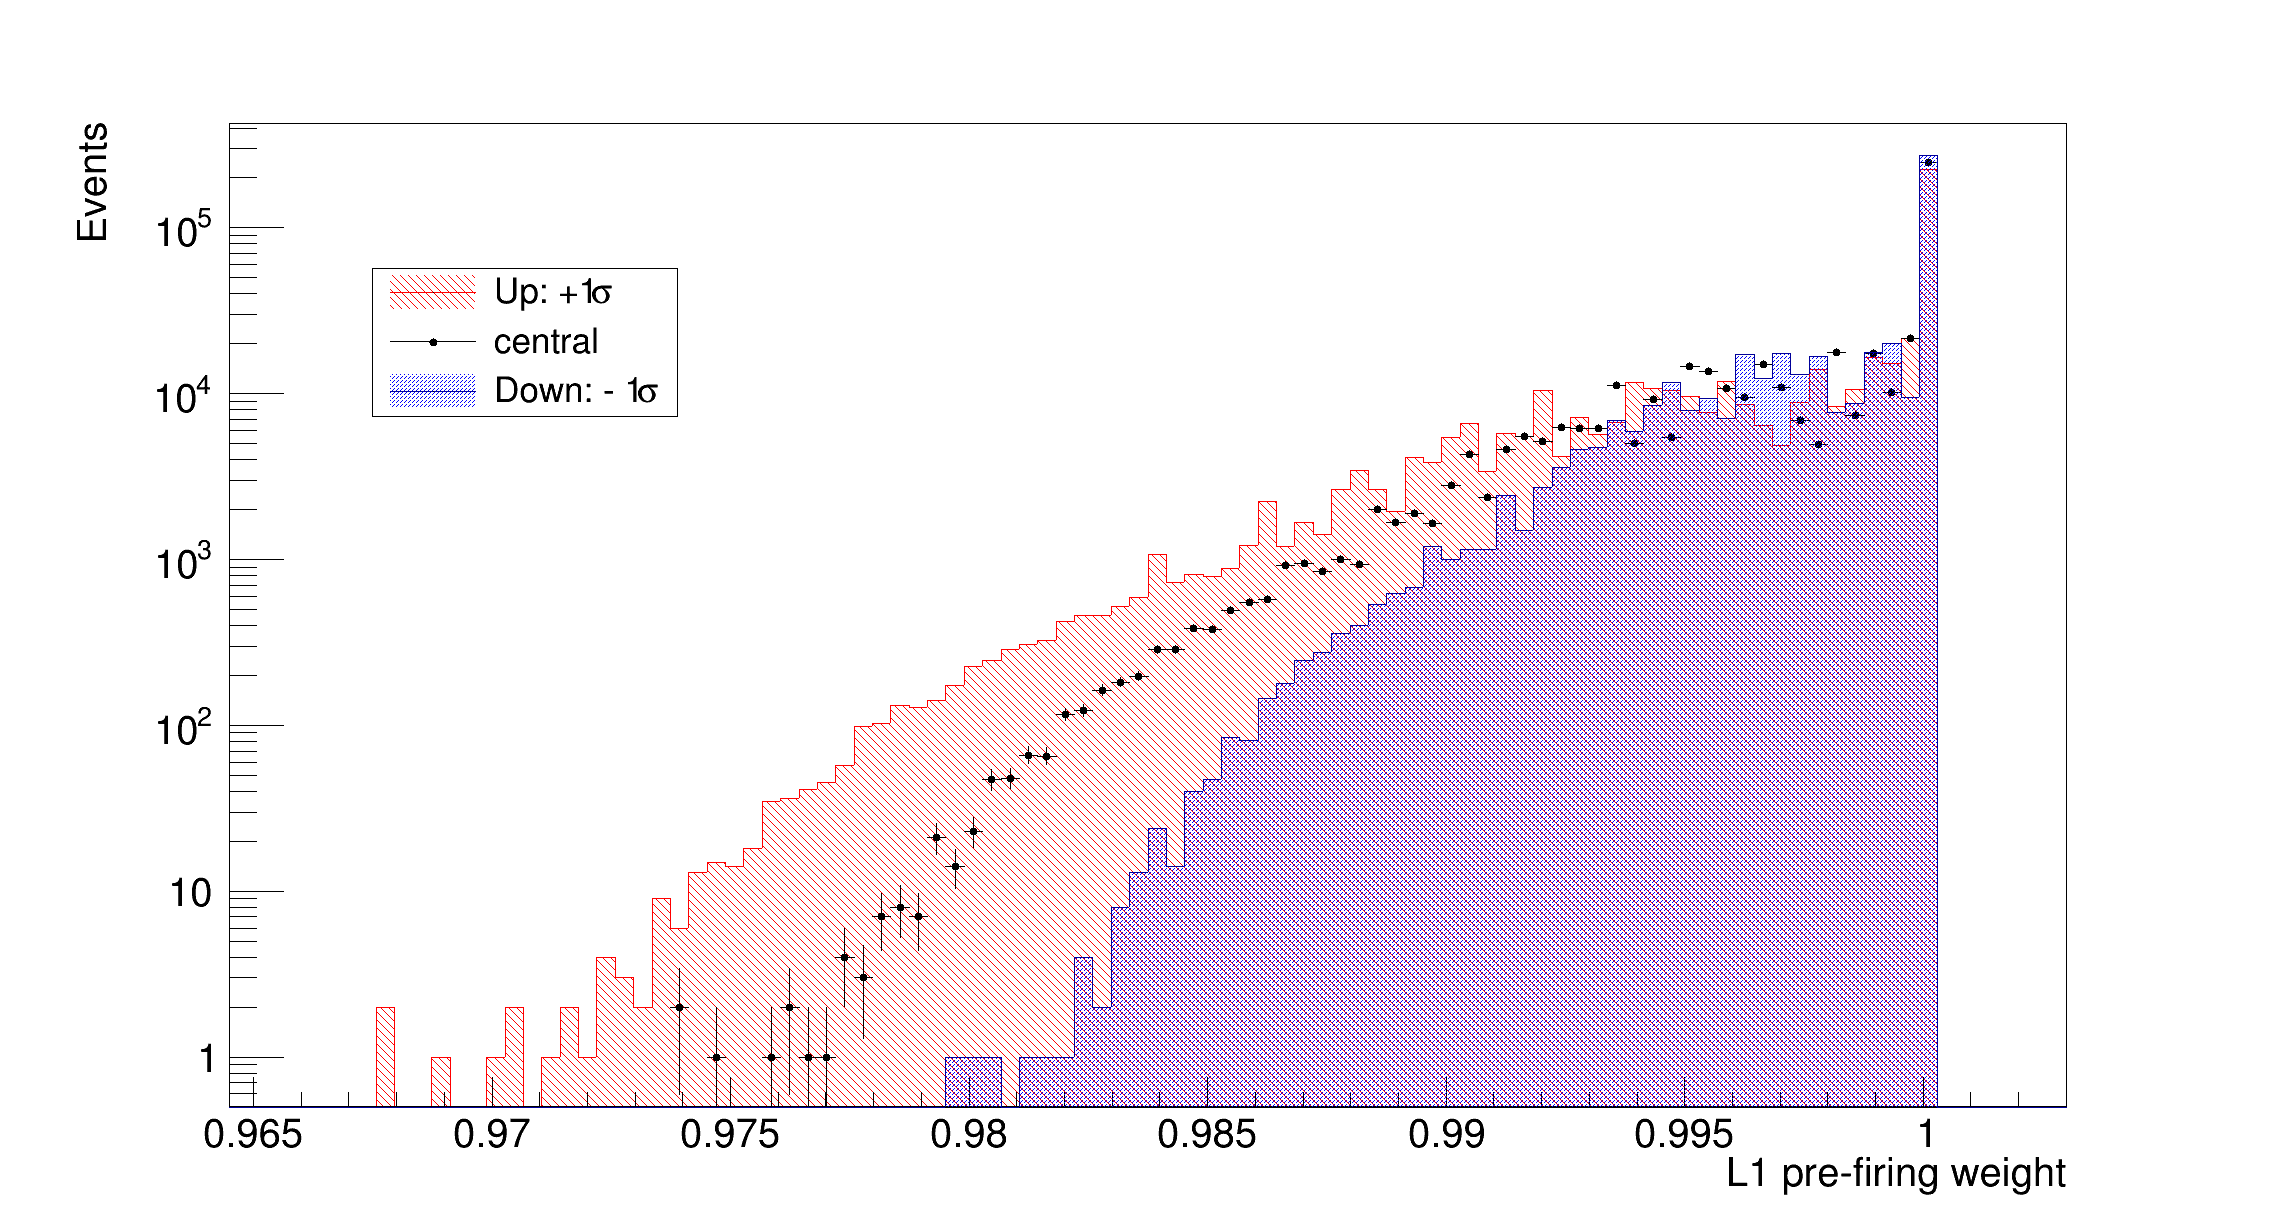
\includegraphics[width=.5\textwidth]{Figures/L1Prefiring_ZZGTo4LG.png}}%
\subfigure [Effect on $m_{4\ell\gamma}$] {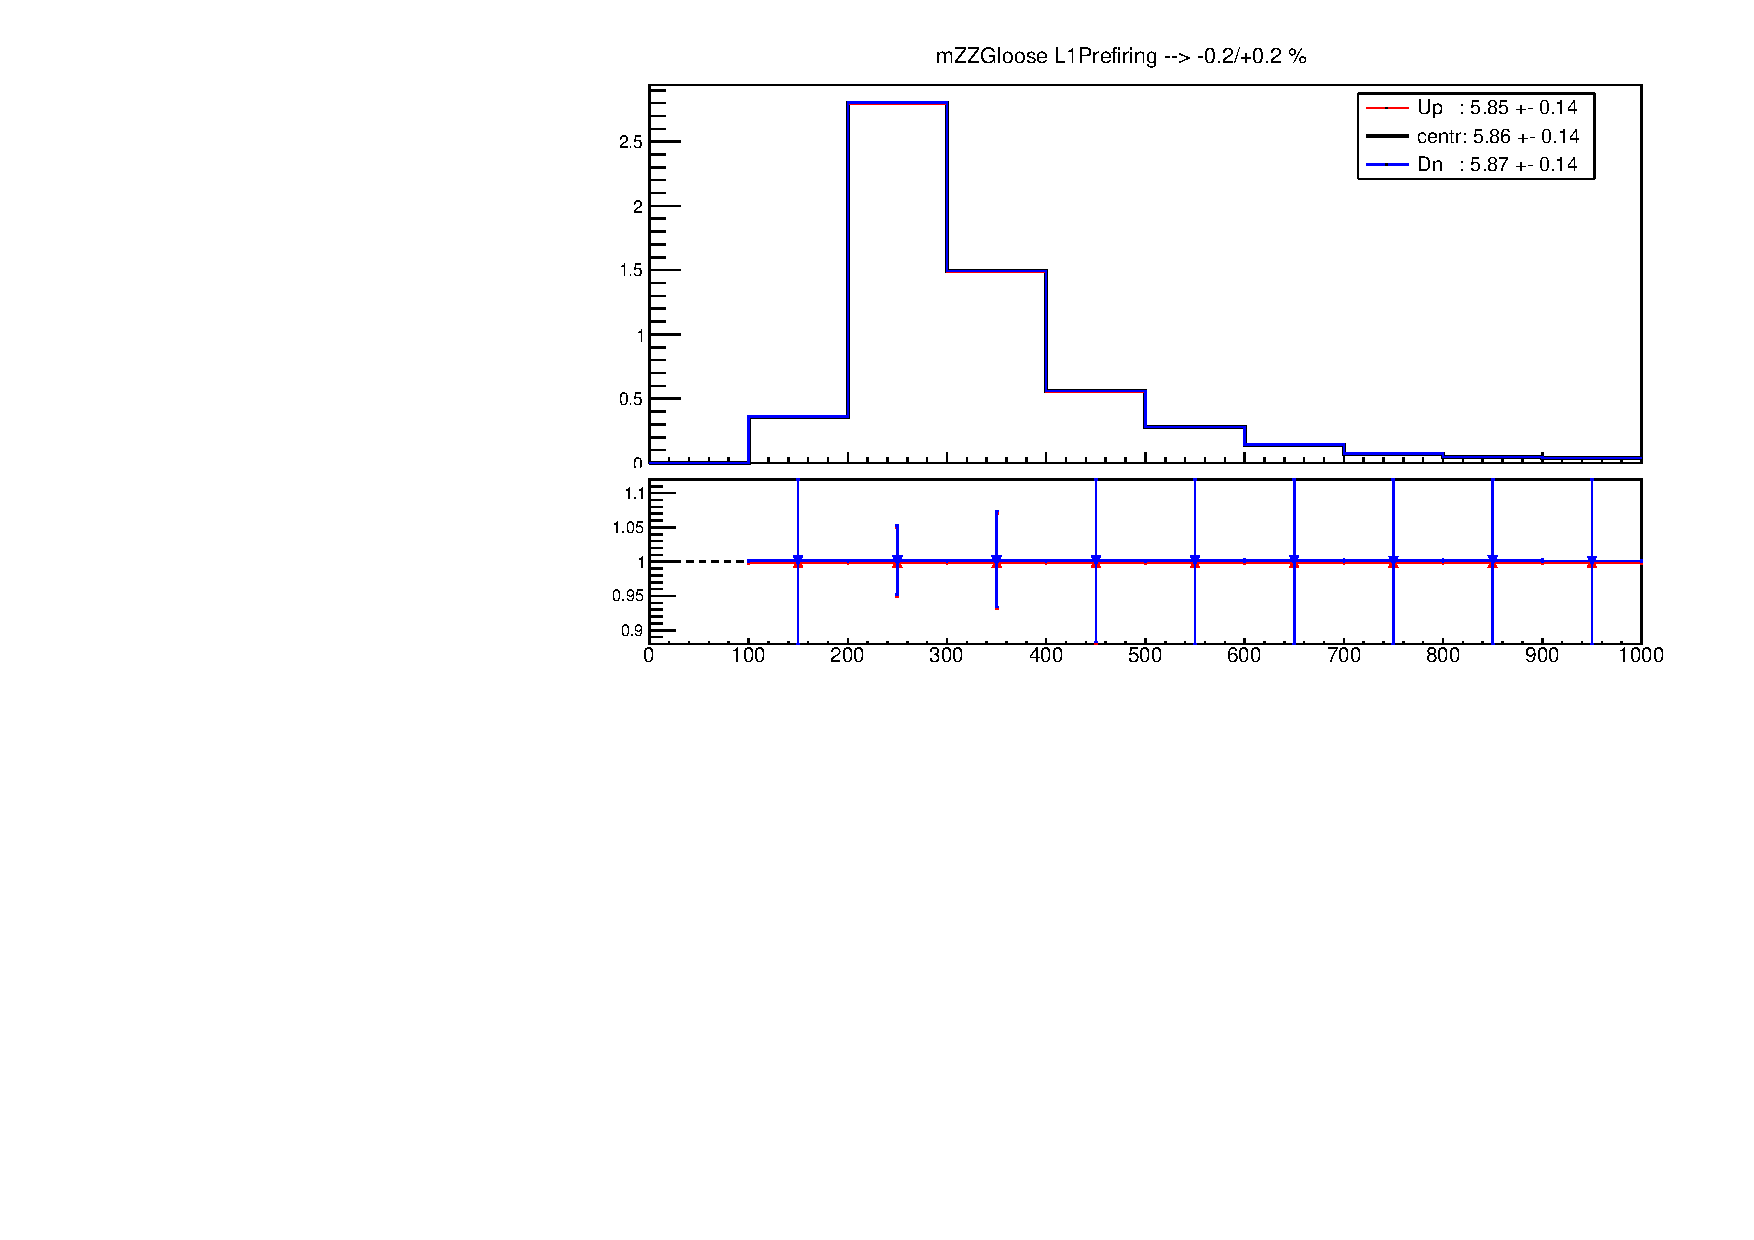
\includegraphics[width=.5\textwidth]{Figures/SYS/SR4P/ZZGTo4LG_mZZGloose_L1Prefiring.pdf}}
\caption{L1 pre-firing weights and their uncertainty on the signal MC in the signal region with four tight leptons and one photon in 2018.
The photon is required to pass the Loose working point of the cut-based ID.}
\label{fig:L1Prefiring}
\end{figure}
